\documentclass[12pt,a4paper]{report}
\usepackage[utf8]{inputenc}
\usepackage{graphicx}
\usepackage{geometry}
\geometry{a4paper, margin=1in}
\usepackage{amsmath}
\usepackage{hyperref}
\usepackage{array}
\usepackage{booktabs}
\usepackage{pstricks}
\usepackage{tikz}

\begin{document}

% --- Title Page ---
\begin{titlepage}
    \centering
    \vspace*{1cm}
    
    {\Large \textbf{A REPORT}}\\[0.5cm]
    {\Large \textbf{ON}}\\[0.5cm]
    {\Large \textbf{PATHFINDER: AI ALTERNATE UNIVERSE\\ GENERATOR}}\\[2cm]
    
    {\large \textbf{BY}}\\[1cm]
    
    \begin{table}[h]
        \centering
        \begin{tabular}{lll}
        Name of the student & ID No. & Discipline \\
        Harshith Bohini & [2024B4A70798H] & [Msc. Math + Computer Science] \\
        \end{tabular}
    \end{table}
    
    \vspace{2.5cm}
    
    {\large \textbf{Prepared in partial fulfillment of the}}\\
    {\large \textbf{Practice School - I}}\\[1.5cm]
    
    {\large \textbf{AT}}\\[1.5cm]
    
    {\large \textbf{[Caarya Innovative]}}\\
    {\large \textbf{A Practice School - I}}\\
    {\large \textbf{Station of}}\\[1.5cm]
    
    {\large \textbf{BIRLA INSTITUTE OF TECHNOLOGY \& SCIENCE,}}\\
    {\large \textbf{PILANI}}\\[0.5cm]
    {\large \textbf{June, 2026}}
\end{titlepage}

% --- Page 2 Form ---
\newpage
\begin{center}
    {\large \textbf{BIRLA INSTITUTE OF TECHNOLOGY \& SCIENCE,}}\\
    {\large \textbf{PILANI}}\\
    {\large \textbf{Practice School Division}}
\end{center}
\vspace{1cm}
\noindent
\begin{tabular}{@{}p{0.45\textwidth}p{0.55\textwidth}@{}}
\textbf{Station} & \textbf{Caarya Innovative} \\[0.5cm]
\textbf{Duration} & \textbf{26 May 2026 to 20 June 2026} \\[0.5cm]
\textbf{Title of the project:} & PathFinder: AI Alternate Universe Generator \\[0.5cm]
\textbf{ID No.(s), Name(s) and} & Harshith Bohini, [2024B4A70798H], [Msc. \\
\textbf{Disciplines of the student(s):} & Math + Computer Science] \\[0.5cm]
\textbf{Name(s) and Designation(s)} & [Dhruv Suman] \\
\textbf{of the expert(s):} & \\[0.5cm]
\textbf{Name(s) of the PS faculty} & [Prof. Swastibrata Bhattacharya] \\
\textbf{member(s):} & \\[0.5cm]
\textbf{Key words:} & AI, Next.js, React, LLM, Generative AI, \\
& Timeline Simulation \\[0.5cm]
\textbf{Project area(s):} & Web Development, Artificial Intelligence, \\
& Human-Computer Interaction \\[0.5cm]
\end{tabular}\\[0.5cm]
\textbf{Abstract:}\\
This report presents the design and development of \textit{PathFinder}, an interactive web application that uses a large language model to generate branching, narratively consistent alternate-life timelines from a user-supplied decision point. The project combines a secure Next.js backend, structured prompt engineering, strict JSON validation, recursive React rendering, and a polished dark-mode interface to transform open-ended user input into an explorable decision tree. Beyond producing creative text, the system emphasizes reliability: the model is constrained to return predictable data, each branch carries probability information, and the frontend visualizes long-range consequences across career, lifestyle, and personality dimensions. The completed prototype demonstrates how generative AI can be framed as a structured reasoning service rather than only a conversational tool.
\vspace{1.5cm}

\noindent
\begin{tabular}{@{}p{0.5\textwidth}p{0.5\textwidth}@{}}
Signature of the student(s) & Signature of the PS faculty member(s) \\[1cm]
Date & Date
\end{tabular}

% --- Acknowledgements ---
\chapter*{Acknowledgements}
\addcontentsline{toc}{chapter}{Acknowledgements}
\par\noindent
I would like to express my sincere gratitude to my mentors at Caarya Innovative and to the Practice School Division of BITS Pilani for providing the opportunity to work on a challenging and contemporary software project. Their guidance helped shape the project from a simple idea into a coherent product with a clear architecture, usable interface, and meaningful application of generative AI. I am also thankful for the technical resources, feedback sessions, and encouragement that supported the development of PathFinder throughout the Practice School period.
\vspace{2cm}

\noindent
Signature of the student(s)

% --- TOC, LOF, LOT ---
\tableofcontents
\listoffigures
\listoftables

% --- Chapter 1 ---
\chapter{Introduction}

\section{Background}
Artificial intelligence applications are increasingly moving from passive chat interfaces toward task-specific tools that can reason, structure, and present information in domain-relevant ways. PathFinder was developed in this context: it is not merely a story generator, but a structured alternate-universe simulation interface. The central idea is based on a common human question: \textit{what would have happened if I had made a different choice?} While no software can predict a life with certainty, a well-designed AI system can help users reflect on possibilities by presenting plausible alternatives, trade-offs, and downstream consequences.

\section{Project Overview}
PathFinder is an AI-powered simulation engine designed to explore ``The Road Not Taken.'' A user enters a past decision point, such as choosing a different college, moving to a new city, changing a career path, or accepting a missed opportunity. The system then acts as a \textit{Timeline Architect}. It expands the decision into multiple branches, assigns relative probabilities, and describes how each path may evolve across career, lifestyle, and personality dimensions.

The project was implemented as a modern web application using Next.js and React. The frontend focuses on an interactive, visual timeline tree, while the backend API route securely communicates with Google's Gemini model. A key engineering concern was that language models naturally produce free-form text, whereas the application requires structured data. Therefore, the project places strong emphasis on prompt design, schema control, JSON parsing, and defensive error handling.

\section{Objectives}
The primary objectives of this project were:
\begin{itemize}
    \item To architect a robust Next.js application capable of handling secure LLM API communication without exposing private credentials to the browser.
    \item To implement a strict JSON schema pipeline for LLM reasoning so that generated outputs can be rendered as reliable timeline trees.
    \item To design and build a premium, responsive user interface featuring an interactive visual representation of alternate life paths.
    \item To ensure that generated narratives show genuine divergence instead of repeating the same outcome with minor wording changes.
    \item To include probability estimates that make the tree more analytical and help users distinguish likely, moderate, and speculative branches.
    \item To refine the application from a prototype-style interface into a more professional product inspired by modern developer tools.
\end{itemize}

\section{Scope}
The scope of the project includes prompt engineering, API integration, frontend component development, responsive UI design, and timeline visualization. The system does not claim to produce scientifically exact predictions. Instead, it offers structured speculative reasoning for reflection, ideation, and creative exploration. Features such as persistent user accounts, database storage, collaborative sharing, and export workflows are identified as future extensions.

% --- Chapter 2 ---
\chapter{Literature Review}

\section{Large Language Models}
Large language models are neural systems trained on large text corpora and capable of generating fluent natural language. In PathFinder, the model is used not only for prose generation but also for structured reasoning. The chosen model, Google's Gemini 2.5 Flash, is suitable for responsive applications because it balances speed, cost, and instruction-following ability. The project leverages the model's capacity to infer plausible consequences while constraining its output to a schema that the application can parse.

\section{Structured Output Generation}
Many generative AI applications fail when model responses are treated as uncontrolled text. PathFinder avoids this by requiring valid JSON with predictable fields. This shifts the model's role from an open-ended narrator to a data-producing service. The schema-driven approach also improves debuggability: malformed responses can be detected, rejected, or retried instead of silently breaking the UI.

\section{Next.js and React}
Next.js was selected because it supports both frontend rendering and backend API routes within one project structure. This reduces deployment complexity and allows the Gemini API key to remain server-side. React was used for componentized rendering of the timeline tree. Recursive components are particularly appropriate for this project because each timeline node can contain child branches with the same shape as the parent.

\section{UI/UX Design Principles}
The project initially used a more experimental visual style with glassmorphism, heavy gradients, and decorative effects. During refinement, the design was shifted toward a professional ``Advanced Human Developer'' aesthetic. This style emphasizes clean typography, minimal surfaces, consistent spacing, solid borders, clear hierarchy, and a pure dark background. The result is a tool-like experience closer to products such as Linear and Vercel than to a novelty demo.

\section{Related Concepts}
PathFinder draws from interactive fiction, decision trees, probabilistic thinking, and human-computer interaction. Unlike a conventional branching game, the user does not select from predefined choices. Instead, the tree is generated dynamically from personal input. This creates a hybrid between storytelling, simulation, and reflective journaling.

% --- Chapter 3 ---
\chapter{Methodology}

\section{System Architecture}
The application is built on a Next.js framework. The frontend consists of React components, notably \texttt{TimelineTree} and \texttt{TimelineNode}, which recursively render the JSON data. The backend is handled by a Next.js API route, \texttt{/api/generate}, which receives the user prompt, constructs the model instruction, calls the Gemini API, and returns parsed data to the browser.

\begin{figure}[h]
    \centering
    % Placeholder for the architecture diagram using TikZ (simplified boxes)
    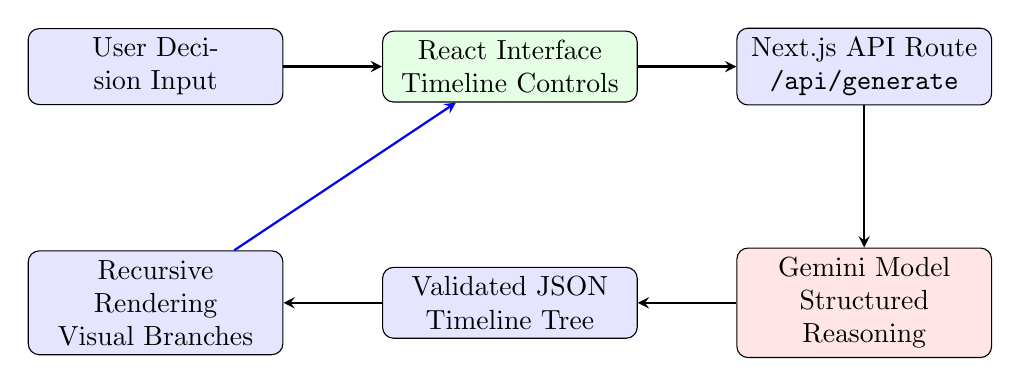
\begin{tikzpicture}[node distance=2cm, auto,
      box/.style={draw, rectangle, rounded corners, fill=blue!10, minimum height=2em, text centered, text width=3cm},
      boxgreen/.style={draw, rectangle, rounded corners, fill=green!10, minimum height=2em, text centered, text width=3cm},
      boxred/.style={draw, rectangle, rounded corners, fill=red!10, minimum height=2em, text centered, text width=3cm},
      arrow/.style={thick,->,>=stealth}]
      
      \node[box] (input) {User Decision Input};
      \node[boxgreen, right of=input, node distance=4.5cm] (react) {React Interface\\ Timeline Controls};
      \node[box, right of=react, node distance=4.5cm] (api) {Next.js API Route\\ \texttt{/api/generate}};
      
      \node[box, below of=input, node distance=3cm] (render) {Recursive Rendering\\ Visual Branches};
      \node[box, below of=react, node distance=3cm] (valid) {Validated JSON\\ Timeline Tree};
      \node[boxred, below of=api, node distance=3cm] (gemini) {Gemini Model\\ Structured Reasoning};
      
      \draw[arrow] (input) -- (react);
      \draw[arrow] (react) -- (api);
      \draw[arrow] (api) -- (gemini);
      \draw[arrow] (gemini) -- (valid);
      \draw[arrow] (valid) -- (render);
      \draw[arrow, color=blue] (render) -- (react);
    \end{tikzpicture}
    \caption{High-level architecture of PathFinder}
\end{figure}

\section{Prompt Engineering and Data Structure}
To ensure that the LLM outputs a renderable tree, a highly structured prompt was developed. The model is instructed to output only valid JSON and to avoid Markdown, explanations, or extra prose outside the object. Each node in the generated tree represents a life stage and includes the following fields:

\begin{itemize}
    \item \textbf{year:} The timeframe of the branch, such as ``Years 1--3'' or ``Years 10--20''.
    \item \textbf{career:} The likely professional development in that branch.
    \item \textbf{lifestyle:} The social, financial, geographic, and daily-life implications.
    \item \textbf{personality:} The possible emotional or behavioral transformation of the user.
    \item \textbf{probability:} A relative likelihood estimate for the branch compared with sibling branches.
    \item \textbf{branches:} A list of child nodes representing further divergence.
\end{itemize}

\begin{table}[h]
    \centering
    \renewcommand{\arraystretch}{1.5}
    \begin{tabular}{@{}p{0.25\textwidth} p{0.7\textwidth}@{}}
    \toprule
    \textbf{Field} & \textbf{Purpose in the Application} \\
    \midrule
    \texttt{year} & Establishes temporal progression and prevents disconnected story fragments. \\
    \texttt{career} & Captures education, work, income, skill growth, and professional direction. \\
    \texttt{lifestyle} & Describes location, relationships, routine, social life, and quality of life. \\
    \texttt{personality} & Adds reflective depth by showing how choices may affect identity and habits. \\
    \texttt{probability} & Provides visual and analytical weight to each possible branch. \\
    \texttt{branches} & Enables recursive generation of long-range alternate timelines. \\
    \bottomrule
    \end{tabular}
    \caption{Core JSON schema fields used by PathFinder}
\end{table}

\section{Frontend Implementation}
The frontend was implemented using reusable React components. The main input form collects the user's decision point and sends it to the backend. Once the response arrives, the timeline tree is rendered recursively. Each node summarizes the life stage and can expand to reveal richer narrative details. Probability values influence visual emphasis so that highly likely paths appear more prominent than speculative ones.

The timeline visualization uses CSS Flexbox for layout, CSS pseudo-elements for connector lines, and CSS Grid for smooth content expansion. Transitions were kept short and intentional, generally around 150 milliseconds, so the interface feels responsive without becoming distracting. The final interface uses dark surfaces, restrained borders, and clear spacing to support long reading sessions.

\section{Backend Implementation}
The backend API route performs four important tasks. First, it validates the request payload to ensure that the input is present and meaningful. Second, it builds a carefully worded prompt that defines the role of the model, the required schema, and the expected depth of the timeline. Third, it sends the request to Gemini using server-side credentials. Finally, it parses the response and returns usable JSON to the frontend.

This separation is important for security and maintainability. The browser never receives the API key, and the frontend does not need to understand the details of model communication. If the model provider changes in the future, the API route can be modified while preserving most of the UI code.

\section{Visual Timeline Model}
The conceptual timeline follows a branching tree. Each decision produces several near-term outcomes, and each of those outcomes can lead to further long-term consequences. Figure 3.2 shows a simplified version of this structure.

\begin{figure}[h]
    \centering
    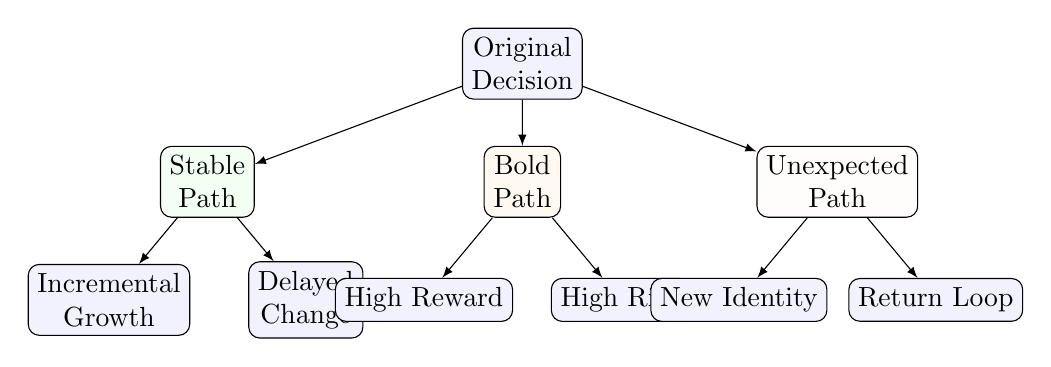
\begin{tikzpicture}[sibling distance=3.5cm, level distance=1.5cm,
      every node/.style = {shape=rectangle, rounded corners, draw, align=center, fill=blue!5},
      edge from parent/.style = {draw, -latex},
      level 1/.style={sibling distance=4cm},
      level 2/.style={sibling distance=2.5cm}]
      
      \node {Original\\ Decision}
        child { node[fill=green!5] {Stable\\ Path} 
          child { node {Incremental\\ Growth} }
          child { node {Delayed\\ Change} }
        }
        child { node[fill=orange!5] {Bold\\ Path} 
          child { node {High Reward} }
          child { node {High Risk} }
        }
        child { node[fill=pink!5] {Unexpected\\ Path} 
          child { node {New Identity} }
          child { node {Return Loop} }
        };
    \end{tikzpicture}
    \caption{Simplified branching timeline model}
\end{figure}

% --- Chapter 4 ---
\chapter{Implementation Details}

\section{Component Design}
The component hierarchy was organized to keep rendering logic readable. A parent component manages application state, including loading status, user input, generated data, and error messages. The tree component receives the generated root node and passes each child node to a reusable node component. This design avoids duplicating rendering logic for different depths of the tree.

\section{Error Handling}
Generative AI systems can fail in several ways: network requests may time out, API keys may be missing, the model may return malformed JSON, or the output may be too shallow. PathFinder accounts for these risks by separating loading, success, and error states in the UI. The backend parsing layer is also designed to detect invalid responses before they reach the visualization layer.

\section{Design Refinement}
One of the most important improvements was the shift from a visually busy prototype to a professional interface. The refined UI uses fewer colors, stronger contrast, and clearer spacing. This matters because the generated content can be dense. A calm interface helps the user compare branches without visual fatigue.

\begin{table}[h]
    \centering
    \renewcommand{\arraystretch}{1.5}
    \begin{tabular}{@{}p{0.25\textwidth} p{0.35\textwidth} p{0.35\textwidth}@{}}
    \toprule
    \textbf{Area} & \textbf{Initial Approach} & \textbf{Refined Approach} \\
    \midrule
    Visual style & Heavy gradients and decorative effects & Minimal dark theme with restrained accents \\
    Motion & Larger animated effects & Short, snappy transitions \\
    Data handling & Model output treated as mostly text & Strict JSON schema and parsing pipeline \\
    Tree display & Prototype-level branch rendering & Recursive components with clearer hierarchy \\
    User trust & Creative but inconsistent feel & Product-like, stable, and readable experience \\
    \bottomrule
    \end{tabular}
    \caption{Major refinements made during development}
\end{table}

% --- Chapter 5 ---
\chapter{Results and Discussion}

\section{Functional Outcome}
The implemented system successfully accepts a user prompt, such as ``What if I moved to Tokyo after high school?'', and generates a plausible branching timeline within a short response time. The output is not a single story but a structured set of alternatives. This makes the application more interactive than a conventional text generator because users can inspect multiple paths and compare their consequences.

\section{User Experience Outcome}
The professional UI significantly improved the perceived quality of the application. The removal of excessive animations in favor of snappy transitions and the use of solid borders on a pure dark background made the application feel like a robust software tool rather than a prototype. The dynamic coloring of nodes based on probability provides immediate visual feedback on the likelihood of different paths.

\section{Technical Outcome}
The project demonstrates that structured prompting is essential when LLM output must drive a user interface. A plain natural-language response would be difficult to render reliably. By converting the model response into a tree-shaped JSON structure, the application can separate generation from presentation. This separation also makes future improvements easier, such as adding export features, saving timelines, or comparing multiple generated runs.

\section{Limitations}
The most important limitation is that the generated probabilities are interpretive rather than statistically verified. They should be treated as narrative estimates, not empirical forecasts. The system is also dependent on the quality of the user's input: vague prompts tend to produce generic timelines, while specific prompts produce richer results. Finally, because the application uses a third-party model API, response time and reliability depend partly on external service availability.

% --- Chapter 6 ---
\chapter{Conclusions and Future Work}
PathFinder demonstrates the viability of using structured LLM outputs to generate complex, interactive narratives. The Next.js architecture proved effective for this use case because it allows frontend visualization and backend API communication to coexist in a single project. The most valuable lesson from the project is that generative AI becomes more useful when it is constrained by product design: schemas, components, validation, and clear interaction patterns turn raw model output into a dependable application experience.

Future work could include:
\begin{itemize}
    \item Implementing user authentication so that generated timelines can be saved and revisited.
    \item Adding a database layer to store prompts, generated trees, and user-selected favorite branches.
    \item Providing an export feature for saving a timeline tree as an image or PDF document.
    \item Allowing users to manually add custom branches or modify the LLM-generated nodes.
    \item Supporting comparison mode, where two alternate decisions can be generated and viewed side by side.
    \item Adding stronger validation or retry logic when model responses do not match the expected schema.
\end{itemize}

% --- Chapter 7 ---
\chapter{Recommendations}
For future projects that use LLMs for structured data generation, rigid schemas should be enforced from the beginning. Prompt instructions should clearly specify output format, field names, nesting depth, and prohibited content such as Markdown wrappers. It is also recommended to keep model calls behind a server-side API route so that credentials remain secure and model-specific code stays isolated.

From a design perspective, a clean interface should be treated as a core feature rather than a final polish step. In AI applications, users must evaluate generated content critically; therefore, readability, hierarchy, loading states, and error feedback directly affect trust. Minimalist UI design, consistent spacing, and clear visual cues can significantly improve the perceived reliability of the system.

% --- Bibliography ---
\begin{thebibliography}{9}
\bibitem{nextjs} 
Vercel Inc. Next.js Documentation. \url{https://nextjs.org/docs}
\bibitem{gemini}
Google. Gemini API Documentation. \url{https://ai.google.dev/docs}
\bibitem{react}
Meta Platforms, Inc. React Documentation. \url{https://react.dev/}
\bibitem{json}
JSON Schema. JSON Schema Documentation. \url{https://json-schema.org/}
\end{thebibliography}

% --- Appendices ---
\appendix
\chapter{Core Generation Logic}
The core logic for communicating with the Gemini model is located in \texttt{app/api/generate/route.js}. It handles the POST request, constructs the structured prompt, calls the model, and parses the JSON response into the tree structure used by the frontend components.

\chapter{Sample Timeline Node}
The following simplified example shows the type of structured node expected by the frontend:

\begin{verbatim}
{
  "year": "Years 1-3",
  "career": "The user enters a new field and builds early skills.",
  "lifestyle": "Daily routines change due to a new city and peer group.",
  "personality": "The user becomes more independent and adaptable.",
  "probability": 42,
  "branches": []
}
\end{verbatim}

\end{document}
